%% Load document class fithesis2
%% {10pt, 11pt, 12pt}
%% {draft, final}
%% {oneside, twoside}
%% {onecolumn, twocolumn}
\documentclass[12pt,final,oneside]{fithesis2}

%% Basic packages
\usepackage[english]{babel}
\usepackage{cmap}
\usepackage[T1]{fontenc}
\usepackage{lmodern}
\usepackage[utf8]{inputenc}
\usepackage{graphicx}



%% Additional packages for colors, advanced
%% formatting options, etc.
\usepackage{color}
\usepackage{microtype}
\usepackage{url}
\usepackage{cslatexquotes}
\usepackage{fancyvrb}
\usepackage[small,bf]{caption}
\usepackage[plainpages=false,pdfpagelabels,unicode]{hyperref}
\usepackage[all]{hypcap}
%\PassOptionsToPackage{hyphens}{url}\usepackage{hyperref}

%% Fix long URLs in DVIs
\usepackage{ifpdf}

%% Source code highlight

\usepackage{floatrow}
\usepackage[chapter]{minted}
\usemintedstyle{trac}
%get caption above code
\floatsetup[listing]{style=Plaintop}
%caption style    
%\captionsetup[listing]{format=listing, singlelinecheck=false, margin=pt, font={bf}}
%\captionsetup[listing]{format=listing}
%fancyvrb frame
\renewcommand{\listingscaption}{Example}


\DeclareGraphicsExtensions{.pdf,.png,.jpg}

\ifpdf
\else
  \usepackage{breakurl}
\fi

%% Packages used to generate various lists
\usepackage{makeidx}
\makeindex

\usepackage[xindy]{glossaries}
\makeglossary

%% Use STAR and CIRCLE signs for nested
%% itemized lists
\renewcommand{\labelitemii}{$\star$}
\renewcommand{\labelitemiii}{$\circ$}

%% Title page information
\thesistitle{RESTEasy integration with Apache Camel project}
\thesissubtitle{Master's thesis}
\thesisstudent{Roman Jakubčo}
\thesiswoman{false} %% Important when using Slovak or Czech lang
\thesisfaculty{fi}  %% {fi, eco, law, sci, fsps, phil, ped, med, fss}
\thesislang{en}     %% {en, sk, cs}
\thesisyear{Spring 2015}
\thesisadvisor{RNDr. Adam Rambousek}

%% Beginning of the document
\begin{document}

%% Front page with a logo and basic thesis information
\FrontMatter
\ThesisTitlePage

%% Thesis declaration (required)
\begin{ThesisDeclaration}
  \DeclarationText
  \AdvisorName
\end{ThesisDeclaration}

%% Thanks (optional)
\begin{ThesisThanks}
I would like to thank to my supervisors RNDr. Adam Rambousek and Mgr. Marek Grác, Ph.D
for providing constant feedback during the preparation of this master’s
thesis. Many thanks goes to all my colleagues and friends from Red Hat that
expressed their valuable thoughts and helped to make this thesis better.

I would also like to thank to my parents and sister for standing behind me the whole time and bear with me and my personality.
\end{ThesisThanks}

%% Abstract (required)
\begin{ThesisAbstract}
The purpose of this master’s thesis is to design and develop new Camel
component by integrating two open-source projects Apache Camel and
RESTEasy. This new component will act as RESTful web service in
the Camel integration framework.
\end{ThesisAbstract}

%% Keywords (required)
\begin{ThesisKeyWords}
Apache Camel, RESTEasy, JAX-RS, REST, RESTful, integration framework, component, web service

\end{ThesisKeyWords}

%% Beginning of the thesis itself
\MainMatter

%% TOC (required)
\tableofcontents

%% Thesis text structured using
%% chapters, sections, subsections, etc.
\chapter{Introduction}
The age we are living right now is also called Information Age, given that we cannot even imagine our lives without modern technologies. They really make our lives much more easier and the most important part is that they are providing us with crucial information. New technologies arise almost every day as IT segment is much more faster, innovative and agile than other segments. New systems created from scratch are very costly and almost never successful. More effective and better alternative is to assemble new systems from existing and proven components. There are various information systems and technologies based on various programming languages containing a lot of information. It is no surprise that there is a need for connecting these systems together and benefit from their already running code to provide business logic. It sounds really nice and simple, but the differences in technologies and programming languages create a real problem in integration between these systems. Also not every system is ready to be connected to others systems because it does not provide the right interface. These are the problems integration frameworks are trying to solve.

Integration frameworks are trying to enable interoperability across platforms, data formats, programming languages, different interfaces and make it simple as much as possible. The integration is hard and difficult, therefore frameworks are trying to find a way to make it straightforward and bring some real benefits for users when using them rather than intimidate them with hard learning process.

One integration framework is Apache Camel project\cite{camel-web}, which is well-known and very popular in the community. Its main benefits are that it is an open source project, developed under Apache with a strong and helping community. Camel was designed to keep up with new emerging technologies by creating a modular project. The core is lightweight and stable. The framework also provides necessary tools for every integration scenario. The framework is also modular which means that new communication protocols can be added to the Camel as new components. This fact helps with keeping the core lightweight. 

The main purpose of this thesis is to create a new Camel component. This component should integrate RESTEasy project\footnote{\url{http://resteasy.jboss.org/}} into the Camel. RESTEasy is an open source project that provides various frameworks for building RESTful Web Services and RESTful Java applications. This component was required through community process as a new feature. There are other components already providing RESTful services in Camel distribution, thus it may not be clear why there is a need for another similar component. RESTEasy is really popular RESTful implementation in JBoss community. It is also primarily used in WildFly application server in which this new component can be very useful.


Camel's community has a specific rule for naming  new components. To follow this rule, the new component is named \textit{Camel Resteasy}.

Quick overview of thesis is as follows. It is divided into five thematic parts. The first chapter
contains introduction, motivation and purpose of the thesis.

The second chapter introduces all the technologies used in the implementation. It tries to provide the most important facts and information about described technologies with links to more detailed sources for further reading.

The third chapter describes analysis and design. It contains diagrams to better illustrate how the new component works inside Camel.

The next chapter describes implementation of the new component created for this thesis. It provides basic description of classes and their purpose. It also explains some specific problems and features of the developed component.

The last chapter is conclusion of the work.


\chapter{Technologies}\label{tech}
This chapter describes technologies used for implementation of \textit{Camel RESTEasy}  component. Each subsection introduces the technology and tries to explain main functionality and common usage.

\section{Apache Camel}
Apache Camel is an open source rule-based routing and mediation framework implemented in Java\cite{java-web}. It is based on the theory of Enterprise Integration Patterns or EIP, described in the book written by Gregor Hohpe and Bobby Wolf\cite{eip}.

Its main focus is on integration and interaction between various applications or systems for which Camel can provide standalone routing, transformation, monitoring. From this point of view Camel may seem like ESB\footnote{ESB - Enterprise Service Bus}, but this is not the case, because Camel does not provide container support or reliable message bus, but it can be deployed into one and create full integration platforms(also know as ESB) like Apache ServiceMix\footnote{\url{http://servicemix.apache.org/}}, JBoss Fuse\footnote{\url{http://www.jboss.org/products/fuse/overview/}}, and JBoss Fuse Service Works. 

Camel has also extensible and modular architecture that allows implementation and seamless plug in support for new protocols. This architectural design makes Camel lightweight, fast and easily extendable for developers.\cite{camel-in-action}

\subsection{The core features}
Camel uses convention over configuration approach to describe given task by domain-specific language (DSL) in declarative way. This way Camel minimizes number of lines of the source code that are needed for implementation of integration scenarios. The key feature, that also helps with this task is usage of theory of EIPs. They are already integrated in DSL and Camel is getting the most from their potential. 

Another fundamental principle of Camel is that it makes no assumptions about the data format. This feature is important because it makes possible for developers to integrate systems together, without any need to convert data to some canonical format. For this way there are no limitations for integrating together any kind of systems\cite{camel-in-action}.

\subsection*{Routing and mediation engine}
One of the core features of Camel is its routing and mediation engine. A routing engine selectively moves a data from one destination to another based on the route's configuration. Users can also define their own rules for routing, add processors to modify the data, filter them based on some predicate and, at the end, decide the final destination for the delivery.

\subsection*{Enterprise integration patterns}
As mentioned before, Camel is based primarily on EIPs. EIPs describe integration problems and their solutions. They also provide some basic vocabulary, but the drawback is that the vocabulary isn't formalized. Camel comes into this with its language describing integration solutions and tries to formalize the vocabulary. There's almost a one-to-one relationship between patterns described in
Enterprise Integration Patterns and the Camel DSL\footnote{\url{http://camel.apache.org/enterprise-integration-patterns.html}}.

Almost all of EIPs that are defined in the book, are implemented as Processors or sets of Processors in the Camel. Processors are used for manipulation of messages between destinations specified in the Camel route.\cite{camel-dzone}



\subsection*{Domain-specific language}
There are few other integration frameworks with DSL and some also have support for describing route rules in XML. However, bonus that comes with Camel is its support for specifying DSLs in regular programming languages as Java, Groovy, Ruby and even Scala. There is also a possibility to describe the route in a XML document. 

\begin{listing}[ht]
	\inputminted[]{java}{sources/java_dsl_example.java}
	\caption{Java DSL definition of the route}

\end{listing}

\begin{listing}[ht]
	\inputminted[]{xml}{sources/xml_example.xml}
	\caption{XML definition of the route }

\end{listing}

\begin{listing}[ht, p!]
	\inputminted[]{java}{sources/scala_example.java}
	\caption{Scala definition of the route }

\end{listing}


\subsection*{Modular and pluggable architecture}
The next feature is the approach to the architecture, which is done in the modular way. This means that Camel can be easily extended to consume data from an endpoint and produce data to some other endpoint. Camel is describing this as developing a new component where each component is responsible for consuming or producing data for some specific endpoint and technology e.g. \texttt{file}, \texttt{HTTP} and many others. When developers want to develop a new component for some unique system and add its functionality to the project, they just need to follow the structure specified by the framework and extend core classes. 

By default, Camel ships with the few most basic components called \textit{camel-core}. This bundle includes 24 components including components like \texttt{bean}, \texttt{file}, \texttt{log}, \texttt{seda} and \texttt{mock}. Plus there are many more components developed by the Apache community and also third-parties\footnote{\url{http://camel.apache.org/components.html}}. There are already created components that can be used for the most common integration scenarios occurring in systems. Some components worthy of note are web services including SOAP\footnote{SOAP -- Simple Object Access Protocol}, REST\footnote{REST -- Representational State Transfer}, JMS\footnote{JMS -- Java Message Service}, specialized JMS component for Apache ActiveMQ\footnote{\url{http://camel.apache.org/activemq.html}} or components for different database connections.


\subsection*{Configuration}
As mentioned before, Camel uses convention over configuration paradigm to minimize configuration requirements, so developers do not need to learn complicated configuration options and can focus on more important things. This is reflected on configuration of endpoints in routes definitions with URI\footnote{URI -- Uniform Resource Identifier} options, as it can be seen on example \ref{uri-option}.
\begin{listing}[ht]
	\inputminted[]{java}{sources/uri.java}
	\caption{URI options configurations}
	\label{uri-option}
\end{listing}

\subsection*{Type converters}
Next feature of Camel, which is one of the top features for Camel community, are built-in automatic converters. Out of the box Camel ships with more than hundred and fifty converters\cite{camel-in-action}. There is also a possibility to create new custom converters for your specific types. Usage of the converter can be seen on example \ref{converter}. The example also demonstrates use of the converter by Camel without user's knowledge in \texttt{getBody()} method and its parameter.

\begin{listing}[ht, p!]
	\inputminted[]{java}{sources/converter.java}
	\caption{TypeConverter invocation}
	\label{converter}
\end{listing}


\subsection*{Lightweight framework}
From the start, the whole framework was designed to be undemanding and lightweight as possible. The core library has only about 1.6 MB and third-party dependencies are kept at minimum. This way Camel can be easily embedded into any platform, which can be e.g. OSGi\footnote{\url{http://www.osgi.org/Main/HomePage}} bundle, Spring application, Java EE application or web application. 

\subsection{Message model}
In previous parts we talked about sending data from one endpoint to another. That is exactly what Camel is doing but in reality it is sending and receiving messages that encapsulate the data. There are two abstraction classes used for modelling messages in Camel, and these are:
\begin{itemize}
\item
\texttt{org.apache.camel.Message} -- the basic entity containing data that is routed in the Camel 

\item
\texttt{org.apache.camel.Exchange} -- special abstraction used in Camel for exchange of messages, that has \textit{in} message and \textit{out} message as a reply

\end{itemize} 

\subsection*{Message}
The \texttt{Message} object represents data that are used by systems to communicate with each other. Messages are sent in one direction from a sender to a receiver. The \texttt{Message} object consists of body, headers and optional attachments. All messages must be uniquely identified with an unique identifier (UID). The format of UID is not guaranteed and it is dependent on the used protocol. If the protocol doesn't have UID scheme, then generic generator from the framework is used.

Headers are name-value pairs associated with the message, similar to HTTP protocol. They provide additional information about the message such as sender identifiers, encoding, content type or authentication parameters. They are stored in a map within the \texttt{Message} object and each name of the header is unique case-insensitive string and the value can be any Java object.

The body represents content of the \texttt{Message} and its type is generic Java Object, so \texttt{Message} can store any kind or type of content. The sender should send body type acceptable by the receiver. If this is not the case then manual transformation inside the route is needed or, more conveniently, type converters are automatically used by the Camel.


\subsection*{Exchange}
The \texttt{Exchange} is defined as message's container encapsulating the \texttt{Message} used during routing. There are various types of interaction between systems and they are supported by the \texttt{Exchange}. These interactions are called message exchange patterns (MEPs) and they are used to specify messaging styles in the property of the  \texttt{Exchange}. This property has to two different messaging styles: one-way and request-response. 

The request-response pattern, \textit{InOut} pattern called in the Camel, is probably the more well-known style because it is used in HTTP-based transport where client requests to retrieve a web resource and it is waiting for the reply from the server. One-way pattern is defined as \textit{InOnly} and is used primarily in JMS where message is sent to the queue and sender does not need any response from the queue. These two types are just the basic ones, furthermore Camel provides few more special cases\footnote{http://tinyurl.com/exchangePattern}.\cite{camel-exchange}

The \texttt{Exchange} is little bit more complex than the \texttt{Message} object and it consists of\cite{camel-in-action}:
\begin{itemize}
\item
Exchange ID -- is unique ID that identifies the exchange and it is also automatically generated by the Camel if ID is not explicitly set.

\item
Message exchange pattern (MEP) -- defines type of messaging style.

\item
Exception -- If an error occurred during routing, then exception is set into this field.

\item
Properties -- various properties of the \texttt{Exchange} used by Camel, similar to headers in \texttt{Message}. The difference is that properties last for the duration of entire exchange and contain global information, whereas message header are specific to the \texttt{Message}. They can be also edited by developers.

\item
In message -- mandatory input message containing request message.

\item
Out message -- optional message containing reply message if the MEP is set to \textit{InOut}.
\end{itemize}


\subsection{Camel's architecture}
This chapter will describe architecture of the Camel from high-level and then takes closer look on some specific concepts. The basic architecture of the Camel is shown in the figure \ref{camelContext} and should help with getting better picture of the runtime known as \textit{CamelContext}.

\begin{figure}[!h]
\centering
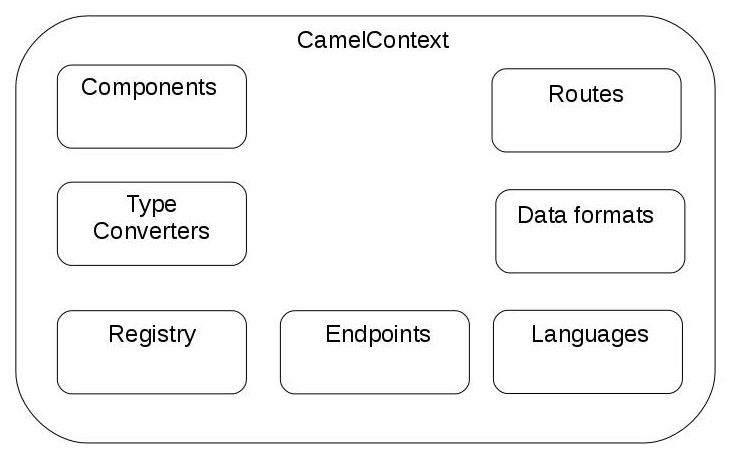
\includegraphics[width=0.9\linewidth]{images/CamelContextCrop.jpg}
\caption{Overview of CamelContext}
\label{camelContext}
\end{figure}

\subsection*{Camel context}
From the figure \ref{camelContext} it is clear that \textit{CamelContext} is similar to container but, more precisely, it is Camel's runtime system. This system keeps everything together and provides services during the runtime that are:
\begin{itemize}
\item
Routes -- routes that have been added to the context

\item
Endpoints -- endpoints that have been created in the context

\item
Components -- components used by the application and they can be added on the fly

\item
Type converters -- loaded type converters by the context

\item
Data formats -- data formats loaded into the context

\item
Languages -- Camel supports different languages used in the expressions and these are loaded into the context

\item
Registry -- registry is used for the look up of beans. JNDI\footnote{JNDI -- Java Naming and Directory Interface} registry is used by default, but if Camel is deployed into Spring or OSGi container then it uses native registry mechanism specific to these technologies.

\end{itemize}

\subsection*{Routing engine and routes}
The routing engine actually moves messages, but is not visible to users. It guarantees correct routing from the sender to the receiver.

The routing engine uses routes for its routing. Routes are the essence of the Camel and are the main and only approach how to specify destination and source for transported information. This means that the route must hold definition of input source to output target. There are many possibilities for definition of the route but the simplest way is to define route as a chain of processors\cite{camel-in-action}. Similarly to messages or exchanges, each route has unique identifier that is used for different operations inside of Camel like monitoring, starting or stopping the route. One of the constraints for the route is the restriction for the number of input sources. Each route must have exactly one input source that is tied to input endpoint and there can be one or several output targets.

\subsection*{Processor}
As mentioned before, the simplest route consists of the chain of processors. The processor represents a node responsible for using, creating or modifying content of incoming exchanges and belonging headers. In the chain of processors, exchanges move during routing from one processor to another in the order defined by the route. Every route can be seen as graph with nodes where output from the one node is input of another.

As stated previously, almost all built-in processors or their combinations are implementation of EIPs but Camel also supports implementation of custom processors and their easy addition to the route.

\subsection*{Component}
Components help with the modular approach and they are main extension point in Camel. Their main purpose and task is to be a factory of endpoints. Developers can create their new components, more information and detail on this topic will be given in subchapter \ref{component-devel}. 

\subsection*{Endpoint}
The endpoint is an abstraction in the Camel that models the end of message channel. In other words it represents sender or receiver. Endpoints are configured and referred in the route using URIs and Camel also looks up the endpoint during runtime by its defined URI. Format of the URI is shown on figure \ref{uri} and it consists of three parts: \textit{scheme}, \textit{context path} and \textit{options}. 

The \textit{scheme} specifies, which component should be used. In the figure \ref{uri} scheme \textit{file} is used that represents Camel \texttt{FileComponent} object that creates \texttt{FileEndpoint}. The component developed in this thesis uses scheme called \textit{resteasy}. The \textit{context path} describes the location of specific resource for the endpoint, similar to a web page address path. The last part of the URI is \textit{options} that is used for specific configuration of the endpoint.

The last task of endpoint is to be factory for creating producers (sender) and consumers (receiver) that are capable of receiving and sending messages in routes.

\begin{figure}
\centering
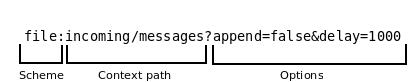
\includegraphics[width=0.9\linewidth]{images/Diagram1.jpeg}
\caption{Overview of endpoint URI}
\label{uri}
\end{figure}

\subsection*{Producer}
Producer is an entity capable of creating and sending a message to an endpoint. Its main task is creating \textit{Exchange} and populating it with content compatible with the endpoint specification. For example, \textit{JmsProducer} will map Camel message to JMS message before sending it to JMS destination. The producer developed in this thesis acts as HTTP client sending HTTP requests using Client API from RESTEasy project.


\subsection*{Consumer} 
As stated before, every route has just one starting point and that is the consumer. The consumer is something like receiver of messages, where the message is sent. Its task is to wrap the message into the \textit{Exchange} and add headers. \textit{Exchanges} created by consumer are then sent and routed in defined chain of processors.

Camel defines two types of consumers: event-driven and polling consumers. The event-driven consumer is probably more known because it is associated with client-server architecture and its communication. In EIPs is this consumer referred also as \textit{asynchronous} receiver and its job is to listen on messaging channel, waiting for the incoming messages.

The polling consumer is working differently than event-driven consumer. It is active consumer that goes to defined address in endpoint and fetches messages from it. Similar to event-driven consumer, polling consumer has different name in EIP world and it is commonly called \textit{synchronous} receiver. This means that all received messages have to be processed before the consumer polls for another one. Common usage of polling consumer in Camel is scheduled polling consumer that checks and polls messages in defined time interval.


 
\section{Development of the new component}\label{component-devel}
Developers can exploit Camel modular architecture and easily extend Camel with new protocols without necessity to change the core of the framework. This feature is achieved by Camel components and by developing a custom component for the protocol. This section describes some of the fundamental principles associated with the creation of the custom component.

Camel is built using Apache Maven\footnote{\url{https://maven.apache.org/}} so the easiest and fastest way to create a custom component from scratch is to use Maven archetype\footnote{\url{https://maven.apache.org/guides/introduction/introduction-to-archetypes.html}}. Camel offers several archetypes\footnote{\url{http://camel.apache.org/camel-maven-archetypes.html}} for different tasks and projects. Archetype \textit{camel-archetype-component} is used for creating a maven project that is a base for developing new components\cite{camel-comp}. 

The created project is fully functional \textit{HelloWorld} demo component containing consumer that generates messages and producer for printing them to the console. Modifying this example is great for creating a custom component. The first thing to do is to decide what name will be used in endpoints for referencing the component. This name must be unique so it does not create conflict with other components. List of the existing Camel components can be found on the official web pages\footnote{\url{http://camel.apache.org/components.html}}

\subsection{Hierarchy of classes}
A Camel component consists of four main classes that together create component and that are \texttt{Component}, \texttt{Endpoint}, \texttt{Producer} and \texttt{Consumer}. The component can have many more classes used for its correct functionality, but only these four are important for creation of correct component in Camel. As stated before, their relationship is that everything starts with \texttt{Component} class, which creates an \texttt{Endpoint}. The \texttt{Endpoint} then creates \texttt{Producers} and \texttt{Consumers}.

Once again, Camel offers some default classes, that can be extended for easier development and not everything needs to be created from scratch.

\subsection*{Component class}
Main job of this class is to be a factory of endpoints. This class needs to implement \texttt{Component} interface and its \texttt{createEndpoint()} method. The easiest way to achieve this is to extend \texttt{DefaultComponent} class. There is also possibility to extend other component classes from other components and leverage theirs functionality.

\subsection*{Endpoint class}
Main task of endpoints is to be a factory for \textit{Consumers} and \textit{Producers}. The \texttt{Endpoint} class needs to implement \texttt{Endpoint} interface that has creation methods for both of them. The simplest way is to extend \texttt{DefaultEndpoint}. Also not all components have to have both \textit{Producer} and \textit{Consumer}. It is common that in some components one of them is not needed or does not make sense in regards to used technology. This class can also contain all parameters that can be set as URI options on the endpoint. Parameters are usually annotated with \texttt{@UriParams} annotation and set though reflection by Camel.

\subsection*{Consumer and Producer class}
The \textit{Consumer} is a starting point through which messages enter the route. Camel offers default implementation for event-driven and polling consumers. This class has no major restrictions how it should be implemented, it just needs to implement \texttt{Consumer} interface with its method \texttt{getEndpoint()}. In the component developed in this thesis, \texttt{ResteasyConsumer} connects to running web servlet and it is consuming requests and responses from the RESTEasy web service. 

The \textit{Producer} is responsible for sending messages outside. Similarly to \texttt{Consumer} class there are no given restrictions on the implementation, it just needs to implement \texttt{Producer} interface, which extends from the \texttt{Processor} interface that has only one method \texttt{process()}. However it is recommended to extend \texttt{DefaultProducer} class to keep it simple\cite{camel-cookbook}. \texttt{ResteasyProducer} acts as HTTP client that sends HTTP requests to specified target.


\section{REST}
For most of the people in modern world, World Wide Web is almost fundamental part of their life and they take it for granted. It is a given fact that Internet has been very successful and it has grown from simple network for researchers and academics to interconnected worldwide community. 

Roy Fielding tried to understand this phenomenon and find out what was the reason or factor for this incredible change in his PhD thesis, Architectural Styles and the Design of Network-based Software Architectures\cite{rest-arch}. In it, he asks three important questions connected with the Web:
\begin{itemize}
\item
Why is the Web so prevalent and ubiquitous?

\item 
What makes the Web scale?

\item
How can I apply the architecture of the Web to my own applications?
\end{itemize}

From answers to these questions, he identifies five specific architecture principles called Representation State Transfer (REST) and these principles are:

\begin{itemize}
\item
Addressable resources -- resource in REST is abstraction of information and data and it must be addressable via URI.

\item
A uniform, constrained interface -- applications should use only a small set of well-defined methods that can manipulate resources.

\item
Representation-oriented -- a resource referenced by one URI can have many different formats, similar to different platforms that need different formats, e.g. HTML\footnote{HTML -- HyperText Markup Language} for web browsers or JavaScript clients needs JSON\footnote{JSON -- JavaScript Object Notation}. The REST application should interact with a service using representations of that service. 

\item
Communicate statelessly -- stateless applications can be scaled more easily.

\item
HATEOAS\footnote{HATEOS -- Hypermedia as The Engine of Application State} -- data formats should drive state transitions in the application.

\end{itemize}

These principles are the reasons, why Web became so successful, enormous and pervasive.\cite{resteasy-book}

\subsection{REST over HTTP}
The REST architecture is not protocol-specific, but it is usually associated with HTTP protocol. The HTTP protocol is primarily used in browser-based web applications, but these applications do not fully leverage all features from it. There are also other web technologies like SOAP that uses HTTP protocol only for transmission and leverages only small fraction of its capabilities. Due to the fact, it may seem like HTTP protocol is not very useful and it has only small set of features. 

In reality, HTTP is very rich and powerful synchronous request/response-based application network protocol with many useful and interesting capabilities for developers. It is used for distributed, collaborative, document-based systems. The protocol works in a simple way, the client sends request message with defined HTTP method to be invoked, headers, location of resource for invocation and it can also contain message body that can be almost anything.

The server handling the request message will send response message with response code, message explaining the code, headers and optional message body. HTTP defines several response codes for different scenarios\footnote{\url{http://www.w3.org/Protocols/rfc2616/rfc2616-sec10.html}}.\cite{resteasy-book}

\subsection{RESTful webservices}
As stated previously, REST was really just explanation for Web's success and growth, but a few years after the publication of Fielding's PhD thesis, developers realized the real potential of REST. They realized that concepts described in the REST architecture can be used for building distributed services and modelling SOAs\footnote{SOA -- Service-Oriented Architectures}. 

SOA is a design pattern that is used for a long time. The simplest description of main concept and idea of SOA is that systems should be designed as set of small reusable, decoupled and distributed services. By combining these services and publishing them on the network, it should be possible to create larger and more complex systems. There were several technologies used for building SOAs in the past like CORBA or Java RMI. Nowadays, most associated technology with SOA are SOAP-based web services.  


\subsection{RESTful architectural principles}
Web services built upon principles of REST architecture are called RESTful web services. These services are used for creating systems based on SOA principles. This section will describe each of the architectural principles of REST in more detail and explain why these principles are important for writing the web service.


\subsection*{Addressability}
The addressability in the systems means that every resource is reachable by the unique identifier. For this, standardized object identity in environment is needed, which is not common in environments. In RESTful services, addressability is achieved by use of URIs and each HTTP request must contain URI of the object requested. The format of URI must be standardized. The format is shown on example \ref{rest-uri}.

\begin{listing}[ht]
	\inputminted[]{bash}{sources/rest-uri.java}
	\caption{URI format}
	\label{rest-uri}
\end{listing}

The format of URI breaks down to six parts where first part is \textit{scheme} that specifies protocol used for the communication, in RESTful web service it is usually \textit{http} or \textit{https}. Next ones are \textit{host} that contain DNS\footnote{DNS -- Domain Name System} name or IP address and optional \textit{port}. These two parts represent a location of the resource on the network. After them is \textit{path} part that specifies a path to the desired resource, similar to directory list of a file on the file system. Last two parts are optional where \textit{query} is list of parameters represented as name-value pairs delimited by "\&" character and \textit{fragment} part is usually used to point to a certain place in the queried document.

\subsection*{A uniform, constrained interface}
To fulfil this principle of REST, the application must only use a finite set of operations of the application protocol on which its services are distributed. When developing RESTful web service, this means only use methods of the HTTP protocol. There are only few operational methods defined on HTTP where each method has specific purpose and these methods are:

\begin{itemize}
\item
\textit{GET} -- a read-only operation used for querying server for specific information. This operation is idempotent, which means that applying this operation over and over will always generate the same result. It also safe in meaning that it doesn't change the state of the server.

\item
\textit{PUT} -- an operation used for storing message body on the server, usually modelled as insert or update. It is also idempotent because sending the same message more than once has no effect on the server.

\item
\textit{DELETE} -- the name is self-explanatory, an idempotent operation for removing resources.

\item
\textit{POST} -- an operation for modifying (updating) the service. It is only nonidempotent and unsafe operation of the HTTP protocol. This means that the request may or may not contain information and also response may or may not contain information.

\item
\textit{HEAD} -- similar to \textit{GET} except no body is returned, only headers and response code.

\item
\textit{OPTIONS} -- an operation for getting information about communication options. Mainly used for getting information on capabilities of the server and a resource without triggering any actions.

\item
\textit{TRACE} and \textit{CONNECT} -- unimportant operations without any use in RESTful web service.
\end{itemize}

Plus constraining interface of web service has few more advantages. One of them is the interoperability. HTTP is ubiquitous protocol and almost all modern programming languages have a HTTP client library. So, it makes sense to expose web services over HTTP, because people will be able to use the exposed web services without any additional requirements. Older technologies have vendor specific client libraries and generated stub codes like \textit{WSDL} files, that creates problem with vendor interoperability in applications. RESTful web services don't have these problems and developers can focus on more important things in the application.

The constrained interface with its well-defined methods have predictable behaviour that can be leverage for a better performance. This means RESTful web services are better in scaling, which is another advantage and that is scalability. RESTful web services are taking the advantage of the caching mechanism of the HTTP protocol. HTTP has very rich configuration for caching semantics that can be used for better performance. So, it is possible to configure caching semantics on defined methods and make the same calls on same clients load much faster because most of the information were cached on the first call. This is use of the same principle as with web pages and browsers. 

\subsection*{Representation-oriented}
The complexity of interaction between client and server in RESTful application is in representations being passed back and forth. Representations can be for almost in any format used in systems, for example XML, JSON, stream, YAML\footnote{YAML -- YAML Ain't Markup Language}. Since RESTful web services are communicating via HTTP, message bodies of requests and responses are acting as representations.

HTTP provides \texttt{Content-Type} header for specification of data formats use between the client and the server. Value of this header is string in MIME\footnote{MIME -- Multipurpose Internet Mail Extension} format, which is very simple: \textit{type/subtype;name=value;}. Where \textit{type} is the main format family and \textit{subtype} is a category. Plus there is a possibility to define name/value properties. Some of the common examples are:

\begin{itemize}
\item
\textit{text/plain}

\item
\textit{application/xml}

\item
\textit{text/html;charset=iso-8859-1}
\end{itemize}

Another feature of HTTP is the possibility for a negotiation of message formats sent between the client and the server, which very useful in web services. There is also a possibility to define a \textit{Accept} header on the client that describes preferred formats of responses. This can be used for the definition of services on the same URIs and same methods but with different return MIME type. Using this, an application can have similar methods but each for a different client with its preferred data format.

\subsection*{Stateless communication and HATEOAS}
Next mentioned principle of RESTful web service is its statelessness, but it means that the application cannot have a state. Stateless in RESTful means that server doesn't store any client session data and instead only manages states of resources it exposes. Session specific data, if they are needed, must be maintained by the client and can be send with the request if needed. This feature can be leverage for easier scaling in clustered environments because only machines need to be added for a scale up. 

The last principle of RESTful web services is HATEOS where the main idea is using Hypermedia As The Engine of Application State (HATEOAS). This approach is very useful because hypermedia have added support for embedding links to other services or information within the document format. One of the uses is for example, aggregating complex sets of information from different sources and using hyperlinks in the document to reference additional information without bloating responses. But the "engine" part is much more useful because it is a different approach from traditional and older distributed applications that have a list of services they know exist. These applications then call central server for a location of these services. Instead of that, RESTful web services with each response returned from a server define new possible interactions that can be done next, as well transition state of the application.

\section{RESTEasy}
RESTEasy is a JBoss project providing frameworks for building RESTful Web Services and RESTful Java applications. This means that it is a fully certified and portable implementation of the JAX-RS specification, which can run in any servlet container. It is also no surprise that it is fully integrated with JBoss Application Server and WildFly to make better experience in that environment. To understand better what exactly is RESTEasy, it is required to understand what exactly is JAX-RS specification.\cite{resteasy-doc}

 
\subsection{JAX-RS 1.0 and 1.1}
RESTful services could be developed in Java for a long time using servlet API, but this approach is really hard and requires lot of code for simple operations. To simplify implementation of RESTful service, a new specification was defined in 2008 called JAX-RS. JAX-RS is a new JCP specification that provides a Java API for RESTful Web Services over the HTTP protocol. This section will just provide some basic information about this specification. The more detailed description and documentation can be found on the official web page of JAX-RS\footnote{\url{https://jax-rs-spec.java.net/}} or on RESTEasy web page\footnote{\url{http://resteasy.jboss.org/}}. 

JAX-RS is a framework that focuses on applying Java annotations introduced in Java SE 5 on plain Java objects. JAX-RS API is part of JSR-311\footnote{\url{https://jcp.org/en/jsr/detail?id=311}}. To simplify development of RESTful Web Services, this framework has annotations to bind specific URI patterns and HTTP methods to individual methods in the basic Java class. It also has parameter injection annotations for easier parsing of information from HTTP requests. Another feature are message body readers and writers for decoupling data format marshalling and unmarshalling from custom Java objects. It also has exception mappers for mapping application-thrown exceptions to HTTP response code and message. The last useful feature  it provides are facilities for the HTTP content negotiation.\cite{resteasy-book}\cite{jax-wiki}

JAX-RS 1.1 is an upgrade version of the same framework with few changes. The biggest one is that it became official part of Java EE 6, which means that no configuration is necessary to start using JAX-RS. Some of the enhancements to the framework include adding examples to clarifying and correcting Javadoc comments related to use of JAX-RS. There was also added a new annotation \texttt{@ApplicationPath}, which can be used to specify base URI for all \texttt{@Path} annotations. Complete list of all changes can be found in the official changelog\footnote{\url{https://jcp.org/aboutJava/communityprocess/maintenance/jsr311/311changelog.1.1.html}}. \cite{jax-1.1}\cite{jax-1.1-2}

It is important to note that both, JAX-RS 1.0 and 1.1 are only server-side specifications without any support for the client side. But this drawback was removed in the version 2.0 and will be described in a more detail in the next subsection.

\subsection{JAX-RS 2.0}\label{jax2.0}
With Java EE 7 release also came new version of JAX-RS 2.0 that upgraded the framework and added new features from which the key features are:
\begin{itemize}
\item
Client API

\item 
Server-side asynchronous HTTP

\item
Filters and interceptors
\end{itemize}

This subsection provides basic overview of the mentioned features. Of course there are other minor features and upgrades to make the framework more useful and stable.

\subsection*{Client API}\label{client-api}
Both previous versions of the JAX-RS specification were missing the Client API, as it was stated previously. Because of this missing feature, each implementation of JAX-RS created their own Client API, which is not so great for the standardized framework. Version 2.0 is correcting this mistake and contains fluent, low-level request building API that can be seen on example \ref{rest-client}. 

\begin{listing}[ht]
	\inputminted[]{java}{sources/client.java}
	\caption{Client API}
	\label{rest-client}
\end{listing}

The base of the API is \texttt{Client} interface that manages HTTP connections and acts also as a factory for \texttt{WebTargets}. \texttt{WebTarget} represents specific URI for a request and the whole request is built and executed on it. In most times the return object is \texttt{Response} from which \texttt{readEntity()} method is used for getting the entity. The API also provides a way to get specific Java object directly without working with \texttt{Response} object as shown on example \ref{rest-client} with the \texttt{Car} object.

The Client API also provides support for asynchronous requests, which can be used for the execution of HTTP requests in the background. There are two possibilities how to get the response and that is either polling or receiving a callback. For polling \texttt{Future} interface is used, which is part of JDK from version 5.0 and client example with \texttt{Future} is shown on example \ref{future} in the appendix. For callbacks \texttt{InvocationCallback} interface shown on example \ref{callback} is used, where the request is registered with the callback instance and is invoked in the background. The interface depending on the status of the response executes a defined code\cite{jax-rs-2.0-new}\cite{jax-rs-2.0}. The client example with callback is shown on example \ref{callbackClient} in  the appendix.

This subsection just gave a quick look on the Client API. For more detail about the Client API check the specification and the Javadoc of JAX-RS 2.0.

\begin{listing}[ht]
	\inputminted[]{java}{sources/callback.java}
	\caption{InvocationCallback interface}
	\label{callback}
\end{listing}

\subsection*{Asynchronous server-side}
A typical HTTP server works in a way that when requests comes in, one thread is responsible for processing and generating response to the client. This is no problem because requests are short-lived, so few hundred threads can handle few thousand concurrent users with good response times. This was fine until evolution of services and HTTP traffic with JavaScript clients. One scenario started to become a problem and that is the scenario where the server needs to push events to the client. In this scenario, clients need to know actual information from the server, for example a stock price, so they usually send \textit{GET} request and just block indefinitely until the server is ready to send back a response. With many clients, this creates large amount of open, long-running requests that are just idling and also threads with them. This scenario is very consuming on operating systems resources and it is really hard to scale up these server-push applications, because JAX-RS had one thread per connection model.\cite{resteasy-book}

To conquer this problem, JAX-RS 2.0 provides a new feature and that is a support for asynchronous HTTP. With it, it is possible to suspend the current server-side request and have different thread handle sending back the response to the client. This feature can be used to implement long-polling interfaces or the server-side push as mentioned. The server-side push problem can be resolved with small set of threads delegated just for sending  responses back to polling clients.

This feature is very analogous to Servlet 3.0 specification and similar to other features of JAX-RS, it is also annotation driven. To use this feature, the application must interact with \texttt{AsyncResponse} interface. This is done by injecting this interface into JAX-RS method with \texttt{@Suspend} annotation.\cite{resteasy-book}\cite{jax-rs-2.0} An example  \ref{async-server} is provided in appendix and more detail information can be found in the specification and the Javadoc of JAX-RS 2.0.

\subsection*{Filters and entity interceptors}
The last notable new feature of JAX-RS 2.0 are filters and entity interceptors. They are used for intercepting requests and the response processing. Notable use cases are authentication, caching or encoding. Similar to the Client API, most implementations of JAX-RS implemented their own interceptors prior to version 2.0. The framework defines two concepts for interceptions and they are:
\begin{itemize}
\item 
filters

\item
entity interceptors
\end{itemize}

Filters are used for the modification or the processing of incoming and outgoing requests or responses. They are executed before and after the request and the response processing. Main task for entity interceptors is marshalling and unmarshalling of message bodies.

In filters, there are two main groups: server-side filters and client-side filters. Both groups have two different filters for the request and  the response. Server-side filters are \texttt{ContainerRequestFilter} that runs before JAX-RS resource method is invoked and \texttt{ContainerResponseFilter} that runs after the invocation of the resource method. An added feature for \texttt{ContainerRequestFilter} is a possibility to specify when the filter should be invoked, before the resource method is matched or after it is matched. This is defined by \texttt{@PreMatching} and \texttt{@PostMatching} annotations. Client-side filters have also two types: \texttt{ClientRequestFilter} and \texttt{ClientResponseFilter} where request filters run before sending the HTTP request to the server and response filters run after receiving response from the server but before the response body is unmarshalled. \cite{jax-rs-2.0}\cite{resteasy-book}

Interceptors deal with message bodies and are executed in the same call stack as their corresponding reader and writer. There are two different types again. One type is \texttt{ReaderInterceptor} that wraps around \texttt{MessageBodyReaders} and the second type is \texttt{WriterInterceptor} that wraps around \texttt{MessageBodyWriters}. They are many uses for these interceptors like implementation of specific encoding, generating digital signatures or posting and preprocessing a Java object before or after it is marshalled.\cite{jax-rs-2.0}\cite{cxf-jax}


%\subsection{Features of RESTEasy}\label{resteasy}


\section{Existing RESTful components}
The official distribution of Camel already provides several components that are used for an integration with RESTful Web Services. There are mainly similar project to RESTEasy and few of them are also certified implementations of the JAX-RS 2.0 specification. Notable examples are:
\begin{itemize}
\item
Camel CXF

\item
Camel Restlet

\item
Camel Spark-rest

\item
Camel Rest
\end{itemize}

Each component and technology has specific pros and cons. Spark-rest is a component integrating Spark Rest Java library running only on Java 8 and supporting the consumer endpoint only. Spark-rest is not a certified implementation of JAX-RS 2.0, but can be used for the server-side. Restlet and CXF components are integrating Restlet and CXF frameworks; both have producer and consumer endpoints along with few unique features. 

The last component is Camel Rest that was added in Camel 2.14. It is used for defining REST endpoints using REST DSL\footnote{\url{http://camel.apache.org/rest-dsl.html}} right in the Camel route. There is also a possibility to configure this component to use some other RESTful component as a base. Any component can be integrated with REST DSL if they have a Rest consumer in Camel. For the integration, the new component must implement \texttt{RestConsumerFactory}. The component then must implement a logic to create the Camel consumer exposing the REST services based on given parameters, such as path, verb, and other options.

\subsection{Camel Resteasy -- motivation}
As for now, Camel already provides RESTful components, so why exactly do we need a new RESTful component if there are components capable to satisfy user's needs. Best answer is probably, because we can. If there are more implementations of the JAX-RS specification, then there should be Camel component for the each one. This way, users are not limited and can choose component for their preferred implementation. 

Another thing to consider is the tight connection between RESTEasy and products like JBoss EAP, JBoss AS or WildFly. All these servers have RESTEasy integrated and are using it out for box. Adding a possibility to also create Camel routes integrated with RESTEasy on these servers can help lot of users who are already familiar with RESTEasy framework. Of course, there is no problem to deploy an application with the CXF implementation and use Camel CXF component but adding another libraries to the runtime is risky because of possible dependencies problems. It is much more safer and easier to just add RESTEasy Camel component and use RESTEasy libraries already deployed in the runtime environment.

%
\chapter{Analysis and Design}
This chapter describes software analysis of the new Camel component, and it is taking into account facts written in the previous chapter. Given that the development of the component is pretty restricted and must follow the base skeleton given by the framework, not every part of software analysis is needed. The most useful part of the software analysis in this scenario are data flow diagrams (DFD). But the first thing to do, is to identify base requirements for the new component, so the analysis starts with identifying these requirements. Next section shows data flow diagram (DFD) that illustrates message flow in Camel. This should also help with understanding how the component will work. 

\section{Requirements}
The purpose of this thesis is to integrate RESTEasy project with Apache Camel framework as defined in the assignment. That means the creation of new Camel component that will be exposing REST interface endpoints in Camel, so basically a REST consumer. Because it should be integrated with RESTEasy project, the exposed endpoints should be configured via JAX-RS annotations provided by the RESTEasy. As mentioned previously, the newest version of RESTEasy is also a fully certified implementation of the JAX-RS 2.0 specification, which means it also provides the Client API that should be used as a Camel producer. This component is required by the community for some time and the requirement is logged in  
the Apache's Jira\footnote{\url{https://issues.apache.org/jira/browse/CAMEL-2983}}.

The assignment is only a basic description of the Camel component so there is no detailed listing of requirements and special features for this component. Therefore, more detailed list of requirements and in some cases even restrictions was composed after the analysis of the RESTEasy project. Also some inspiration came after analysis of similar components providing REST endpoints. This is a quick overview of defined requirements and default features for both, the consumer and the producer.

\subsection{Consumer}
The consumer should have these features:

\begin{itemize}
\item
ability to create a consumer connected with defined REST Web Service by RESTEasy (\textit{Basic Consumer})

\item
ability to create a consumer defined only in the route (\textit{Camel Proxy Consumer})

\item
ability to define REST Web Service as an interface with RESTEasy annotations with a consumer in the route and creating responses via route (\textit{Proxy Consumer})

\item
possibility to define allowed request methods for a consumer defined only in the route


\item
ability to change a response returned from REST Web Service in the route, before it is sent to the client 

\item
both request and response should be routed into the route

\item
DSL and Spring support


\end{itemize}

\subsection{Producer}
The producer should have these features:
\begin{itemize}
\item
send a HTTP request to a defined target using RESTEasy Client API

\item
provide the possibility for the basic authentication with URI options

\item
ability to use RESTEasy Proxy Framework Client API (more detail will be given in chapter \ref{producer})

\item
DSL and Spring support
\end{itemize}

\section{Camel's data flow}
This section contains several DFDs illustrating data flow incoming into the Consumer and outgoing from the Producer. 

As defined in the previous section, the new component provides three types of consumers. Each of them has a little bit different data flow, so to understand them better, there are three different diagrams. The first diagram shown on the figure \ref{dfd-basic} shows basic consumer data (message) flow where RESTEasy first process a HTTP request and create a response according to the implementation of the service without sending it to the client. Afterwards, the response is sent to the route as \texttt{Exchange} for another processing. The HTTP request is also bundled into the \texttt{Exchange} in a special header. Once the processing  is done, the final Response is returned to the client. 


The second diagram shown on the figure \ref{dfd-camel}, depicts data flow of the second type of consumer. This is a consumer which being internally called \textit{Camel Proxy Consumer} in this thesis. This type of consumer is defined only in the route, that is exposing it as a web service. The request should be processed in the route along with the creation of the response for the client. This consumer is just a bonus feature; it can be used for the creation of the simple web service without need to create a class with JAX-RS annotations. 


Next diagram shown on figure \ref{dfd-proxy} illustrates the last possible consumer in the new component, which is internally called \textit{Proxy Consumer}. In this type of the consumer, users only have to define an interface with desired methods annotated with JAX-RS annotations. RESTEasy will take care of processing and matching HTTP request, which is afterwards sent for the processing as exchange into the route. The response should be created in the route.  


The final diagram shown on figure \ref{dfd-prod}, depicts message flow in a producer. The producer message flow is reverse to the consumer message flow. It processes exchanges from the route and send the HTTP request to the target. 


\chapter{Implementation}\label{impl}
As stated before, the goal of this thesis is to integrate Apache Camel and RESTEasy to create a new \textit{Camel Resteasy} component. This chapter describes the source code and the implementation of the \textit{Camel Resteasy} component. 

The implementation was done in the Java programming language, similarly to the Camel core and other components. It was also implemented with regards to restrictions set by the Camel framework for components mentioned in previous chapters. Versions that were used in the source code:
\begin{itemize}
\item
Java 1.7

\item
Apache Camel 2.14.0

\item
RESTEasy 3.10.0
\end{itemize}

\section{Class diagram}
The final fully exported class diagram for the \textit{Camel Resteasy} component can be found in the appendix on page \pageref{class-bla}. Sections describing single classes of the component will use only single class diagrams.

\section{ResteasyComponent class}
The \texttt{ResteasyComponent} class is the base of the whole implemented component and it is where everything starts. It extends \texttt{HttpComponent} to leverage already implemented code needed to run in the Camel, after all Resteasy component is similar to \texttt{HttpComponent} because it consumes HTTP requests. As it was already mentioned, the main purpose of \texttt{Component} class is to be a factory of endpoints. Therefore, \texttt{createEndpoint()} method must be implemented and it must override the same method from the \texttt{HttpComponent} class.

There is nothing special about the implementation of this method. The first thing it does is that it reads all the configuration URI parameters and removes them to prevent mistakes in matching them as query parameters. The Endpoint URI is then parsed from the rest of the cleaned URI.

There are two more methods that override methods from \texttt{HttpCom\-ponent}. These methods are \texttt{connect()} and \texttt{disconnect()}. They are used for connecting and disconnecting consumers from \texttt{HttpRegistry}. More about this class see in section \ref{registry}. 

This class also implements the \texttt{RestConsumerFactory} interface to support configuration of the route and options in REST DSL. To implement this interface, the method \texttt{createConsumer()} must be implemented. This method just parses the REST configuration from DSL and creates the endpoint belonging to this configuration.

The \texttt{ResteasyComponent} has also one special property that can be set when creating component in the Camel context. The name of the property is \texttt{proxyConsumersClasses} and it is a string property that can be set to fully qualified names of Java interfaces annotated by JAX-RS annotations separated by comma. More detail about this property and its usage will provided in section \ref{servlet}.

\begin{figure}[h]
\centering
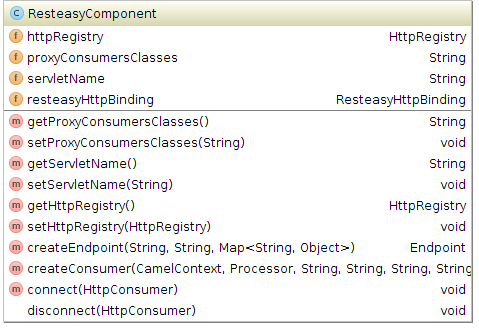
\includegraphics[width=0.8\linewidth]{images/component.png}
\caption{ResteasyComponent class}
\label{comp}
\end{figure}

\section{ResteasyEndpoint class}
\texttt{ResteasyEndpoint}  is straightforward class that is used as a factory for creating \textit{consumers} and \textit{producers} for the Resteasy component. Therefore, there are two methods for this purpose, \texttt{createConsumer()} and \texttt{createProducer()}. These methods are self explaining, so there is nothing to add. This class also extends \texttt{HttpEndpoint}, to leverage a already implemented code that is used in the consumer part of the component.

This class also holds all configuration parameters that were parsed in \texttt{ResteasyComponent}. Parameters are annotated with \texttt{@UriParam} for easier setting using Java Reflection API. The full list of parameters and their basic description is given in the next subsection.

\begin{figure}
\centering
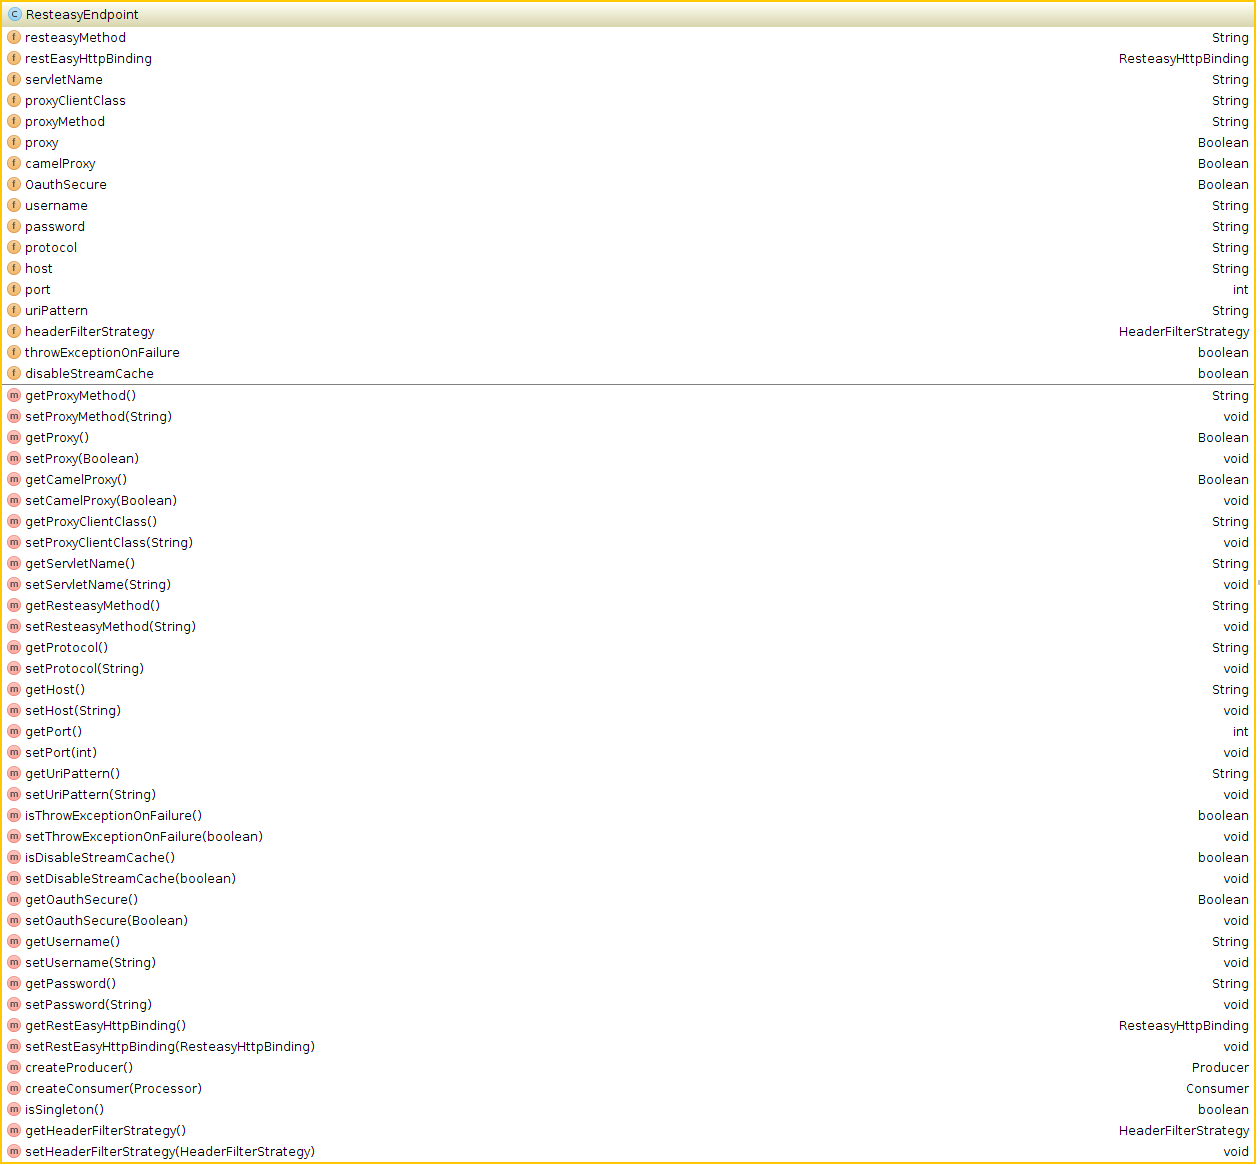
\includegraphics[width=0.9\linewidth]{images/endpoint.png}
\caption{ResteasyEndpoint class}
\label{endpoint}
\end{figure}

\subsection{Parameters}
There is not a lot of configuration parameters for this component, but few of them are unique, so the list of parameters also provides a basic description for each. Also some parameters are specific only for \textit{consumer} or \textit{producer}, which will be noted also in the list. This list contains some options for that it could be hard to understand their meaning or purpose, just from the short description. More detail about their meaning and usage will be provided in sections \ref{consumer} and \ref{producer}, depending if they are \textit{consumer} or \textit{producer} options.  

List of URI parameters for the endpoint:
\begin{itemize}
\item
servletName -- specifies the servlet name that the endpoint will bind to. This name should match the name of the servlet that maintains REST services and it is defined in the \texttt{web.xml} file. This option is for the \textit{consumer} only and it is a required option. 

\item
resteasyMethod -- used to define, which HTTP method should be used in the HTTP client. This option is for the \textit{producer} only. This option can also be specified in \textit{CamelResteasyHttpMethod} header, which also overrides this URI option.

\item
resteasyHttpBindingRef --  reference to an \texttt{ResteasyHttpBinding} in the Registry. \texttt{ResteasyHttpBinding} can be used to customize how a producer works with requests and responses.

\item
proxyClientClass -- option that is used only in the \textit{producer} and it is used for the definition of the name of the proxy class used in the client proxy call.

\item    
proxyMethod -- option required if \textit{proxyClientClass} is specified, therefore only usable in the \textit{producer} endpoint. This option is used for the definition of the name of the method, that should be invoked in the class specified in \textit{proxyClientClass} option.

\item
proxy -- boolean option that can be used only on the \textit{consumer} endpoint. If set to true, then Camel will register this \textit{consumer} as a proxy. 

\item 
camelProxy -- if set to true, then this address is only specified in a route. Can be used only on the \textit{consumer} endpoint.

\item
username -- username for the basic authentication on the \textit{producer} endpoint.

\item
password -- password for the basic authentication on the \textit{producer} endpoint.

\end{itemize}


\section{Resteasy Consumer}\label{consumer}
The \textit{consumer} part is an essential part of this component, because it is really the most useful part of the integration between Apache Camel and RESTEasy. It is also in this part where \textit{Camel Resteasy} component is different in some way compared to other components. The most important thing to note is that RESTEasy doesn't provide any other way how to create a RESTEasy server other than create \texttt{web.xml} file in the application. In this file  servlet for RESTEasy must be specified, which also provides its own servlet class named \texttt{HttpServletDispatcher}. In contrast, other implementations of the JAX-RS specification, like CXF or Restlet provide a way to create their own servers programmatically or as a bean in Spring or OSGi.

\begin{figure}[!h]
\centering
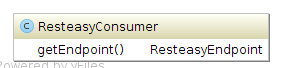
\includegraphics[width=0.6\linewidth]{images/consumer.png}
\caption{ResteasyConsumer class}
\label{fig-consumer}
\end{figure}

Therefore, components based on these projects, usually create the server in their \textit{consumer} class and handle requests along with their integration with Camel. Something similar cannot be done with RESTEasy and that is why is \texttt{ResteasyConsumer} class is so simple as seen on figure \ref{fig-consumer}. Basically this class just acts as a proxy \textit{consumer} class, so Camel knows that there exists a \textit{consumer} for this component.

As a reminder, the component defines three types \textit{consumers}:
\begin{itemize}
\item
\textit{Basic Consumer} -- fully implemented class with JAX-RS annotations and defined path in the \textit{consumer} endpoint

\item
\textit{Proxy Consumer} -- only interface with JAX-RS annotations that must be specified in component property \textit{proxyConsumersClass\-es}. The \textit{consumer} endpoint with this \textit{consumer} has to have \texttt{proxy} option set to true. 

\item
\textit{Camel Proxy Consumer} -- just specified path on \textit{consumer} endpoint with the base URI provided by the servlet. The \textit{consumer} endpoint with this \textit{consumer} has to have \textit{camelProxy} option set to true. 
\end{itemize}


\subsection{ResteasyCamelServlet class}\label{servlet}
\texttt{ResteasyCamelServlet} is the real \textit{consumer} in the Resteasy component. It is extending \texttt{HttpServletDispatcher} class from RESTEasy and acting as a servlet. There are few methods and the most important is \texttt{service()}. This method is responsible for handling requests, creating responses, sending them both to the route and sending the final response back to the client. It also takes into account all configuration options on URI, so it takes care of all three types of consumers in a specific way. 

The \textit{Basic Consumer} takes into account that there exists a fully implemented web service registered in the servlet runtime. So the request for this \textit{consumer} is first handled by the servlet extended by the \texttt{ResteasyCamelServlet} and the response is returned. If the request was invalid, then the created response from the service is returned. If the request was correct, then the response is set as a \textit{exchange} body and sent for the processing into the route. When the processing is done, then the final response is sent back to the client. 

The \textit{Proxy Consumer} works in similar way. One difference is that if the request was correct then the status code 204 is returned. This code means there was no problem with the request but there is no content for the response\cite{http}. That is a correct behaviour because only the annotated interface was provided. In this scenario the request body in set as a \textit{exchange} body and it is sent for the processing into the route. The response should be created in the route, so it can be returned back to the client.

\begin{figure}[h]
\centering
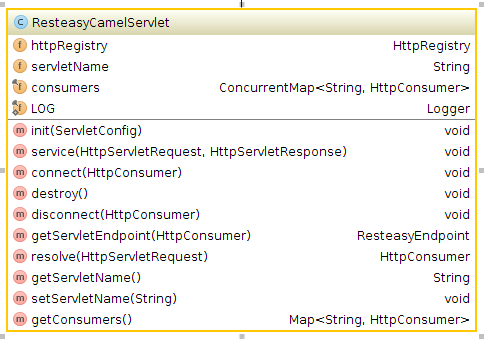
\includegraphics[width=0.8\linewidth]{images/servlet.png}
\caption{ResteasyCamelServlet class}
\label{comp}
\end{figure}

The last type of the consumer is \textit{Camel Proxy Consumer}. This consumer skips the part of handling the request to the extended servlet, otherwise it is working exactly in the same way as the \textit{Proxy Consumer}.     

Another important method is \texttt{init()}, which is used for the creation of \texttt{ResteasyCamelServlet} and registering it in the HTTP registry. The description of the HTTP registry and \texttt{HttpRegistry} class will be provided in section \ref{registry}. This method is also responsible for the \textit{Proxy Consumer}. This special \textit{consumer} was invented as a bonus feature for the component, for scenarios where the response to the request can be created in the route with data from some others systems integrated with Camel. This means that the user doesn't need to implement a full RESTful service but he just needs to create a interface with JAX-RS annotations. This scenario can be very useful to some users but there is a problem with RESTEasy that  does not register just interfaces with annotations. RESTEasy registers interface with annotations only if there is also a class implementing this interface. This problem is solved in \texttt{init()} method with use of the Java Reflection API\footnote{\url{http://docs.oracle.com/javase/tutorial/reflect/index.html}}. If the user wants to use this feature, he must specify created interfaces in \textit{proxyConsumersClasses} property on the \texttt{ResteasyComponent}. The \texttt{init()} method parses these interfaces and using the Reflection API creates dynamic proxy classes\footnote{\url{http://docs.oracle.com/javase/7/docs/technotes/guides/reflection/proxy.html}} for them. These dynamic proxy classes are then registered into the RESTEasy runtime as new resources.

There are few more methods in this class but there are really straightforward. The \texttt{resolve()} method is used for resolving which \textit{consumer} should handle the request. Methods \texttt{connect()} and \texttt{disconnect()} are used for connecting and disconnecting \textit{consumers}. 


\subsection*{ResteasyFilter class}
\texttt{ResteasyFilter} is a class annotated with \texttt{@Provider} annotation and implementing \texttt{Filter} interface. The annotation takes care of registering the filter into the servlet without need to be specified in the \texttt{web.xml} file. This filter doesn't do anything special. Its main task is just wrapping requests and responses into custom wrappers created in the component. This must be done because bodies of requests and responses need to be processed and read more than once in \texttt{ResteasyCamelServlet} to be fully integrated with Camel.

For this purpose, two wrappers \texttt{ResteasyHttpServletRequestWrap\-per} and \texttt{ResteasyHttpServletResponseWrapper} were created. Their main task is to create a copies of bodies of requests and responses, so  \texttt{ResteasyCamelServlet} can manipulate them much more easily.





\subsection{HttpRegistry class}\label{registry}
\texttt{HttpRegistry} is a sort of helping class for consumers in this component. It is primarily used in \texttt{ResteasyCamelServlet} and \texttt{ResteasyComponent} for connecting and disconnecting \textit{consumers}. In short, \texttt{HttpRegistry} interface keeps track of running \texttt{ResteasyServlets} and \texttt{ResteasyConsu\-mers} belonging to them.  To be able to do that, it provides methods for registering and unregistering servlets and \textit{consumers} from the registry.

The Resteasy component also provides a default implementation of this interfaces, \texttt{DefaultHttpRegistry}. This default implementation is used as a default in the component. 

\begin{figure}[!h]
\centering
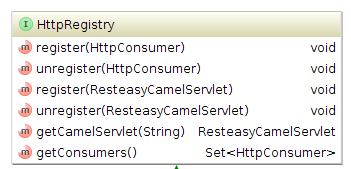
\includegraphics[width=0.8\linewidth]{images/registry.png}
\caption{HttpRegistry interface}
\label{comp}
\end{figure}


\section{ResteasyProducer class}\label{producer}
\begin{figure}[h]
\centering
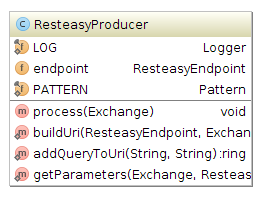
\includegraphics[width=0.6\linewidth]{images/producer.png}
\caption{ResteasyProducer class}
\label{comp}
\end{figure}

\texttt{ResteasyProducer} represents a client part and is implemented using the Client API provided by RESTEasy. It extends \texttt{DefaultProducer} and it is overriding the \texttt{process()} method. There are also few methods  primarily used as helping methods, for creating the right URI, adding a query or getting producer configuration options specified in the URI of the endpoint. The main task of the \textit{producer} is getting data from \textit{exchanges} and sending the HTTP request to the specified target in the endpoint. This is the task of \texttt{process()} method. 

The RESTEasy implementation of the Client API has one bonus feature compared to the common JAX-RS Client API. Of course, it is providing the same basic HTTP client mentioned in chapter \ref{client-api}. The additional feature is RESTEasy Proxy Framework\footnote{\url{http://docs.jboss.org/resteasy/docs/3.0.9.Final/userguide/html_single/index.html\#d4e2143}}. It is the mirror opposite of the JAX-RS server-side specification, meaning the client framework builds a HTTP request that it uses to invoke on a remote RESTful web service. This service also doesn't have to be a JAX-RS service but can be any web resource accepting HTTP requests. To use this client, the user must create a Java interface with JAX-RS annotations on methods and then use the Client API capable invoking proxy methods on the specified interface\cite{resteasy-doc}. More detail about this feature can be found in the RESTEasy documentation. 

To use this feature in the component, the user must specify the created interface with a fully quantified name in the URI option \textit{proxyClientClass} and provide which method of the interface should be invoked in the URI option \textit{proxyMethod}. In reality \texttt{process()} method doesn't have any client logic implementation in it. Its task is to just select that type of the client will be executed depending on the provided configuration of the endpoint. The real implementation logic of transforming \textit{messages} to HTTP requests and HTTP response to \textit{messages} is done in the implementation of the \texttt{ResteasyHttpBinding} interface. The implementation also implements the creation of the client request and its execution.




\section{ResteasyHttpBinding class}
As already mentioned, the \texttt{ResteasyHttpBinding} interface and its implementation \texttt{DefaultResteasyHttpBinding} are responsible for the conversion of \textit{messages} to HTTP requests and HTTP responses to \textit{messages}. It is used only in the \textit{producer} class. 

\begin{figure}[!h]
\centering
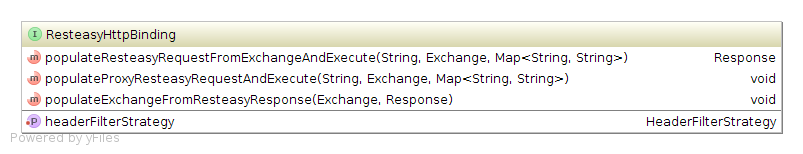
\includegraphics[width=1.0\linewidth]{images/binding.png}
\caption{ResteasyHttpBinding interface}
\label{comp}
\end{figure}


These classes contain only four methods where one is just a setter. There is one method for populating \textit{exchange} from HTTP response and two methods for populating HTTP request from \textit{exchange}, depending if the basic client is used or the proxy one. The important aspect of the transformation between Exchanges and HTTP requests and responses is that all headers are extracted and stored between these objects. This is done in both ways of the transformation. Headers are also all filtered by the given strategy. The component provides a default strategy for the filtration named \texttt{ResteasyHeaderFilterStrategy}, but users also can create their own strategy and set on the endpoint as a URI option.

There is also a possibility to create own implementation of \texttt{Resteasy\-HttpBinding} and set it in the component instead the default one provided by the component. This gives user more flexibility if there is some special task that needs to be done and the default implementation can't handle it correctly.  


\section{Unit tests}
RESTEasy can only run in the container where the \textit{.war} application is deployed and the servlet is created. This is most crucial for the consumer part of the component, so for testing purposes the component was integrated with Arquillian test framework\footnote{\url{http://arquillian.org/}} to use embedded WildFly 8.2 server in tests. Where each test class starts its own WildFly server and deploys a created bundle containing the new component and Camel routes.  

Some units test also leverage \texttt{CamelTestSupport} class that provides lot of useful methods for testing Camel components. This is mostly done in \textit{producer} tests in which Arquillian is integrated \texttt{CamelTestSupport}. Tests also provide example of different definitions of routes in XML or in Java language.

Camel has a convention for the structure of unit tests in which every test class represents a scenario and has a descriptive self-explaining name. This is done to be much more understandable and clear for the outside user. 

%\section{Examples of usage}
%???

\chapter{Conclusion}
The main task of this master's thesis was the integration of RESTEasy project with Apache Camel project. This means designing and developing a new Camel component that should be used for the integration of the RESTful Web Service and the Camel framework. Another requirement set by the thesis description was to provide unit tests. Author should also cooperate with the community, develop new Camel component by project development standards and investigate the RESTEasy implementation. The thesis should also provide comparison of JAX-RS 1.1 and JAX-RS 2.0 specifications.

The result of this master's thesis is Camel Resteasy component. This new component can be used to connect exposed RESTful Web Service to the Camel Consumer. Furthermore, component's Producer can be used as HTTP client that is based on RESTEasy Client API. Thesis also provides comparison between JAX-RS specifications that can be found in the chapter \ref{tech}. 

The source code of the component is included in attachments to this thesis. The source code was also hosted on GitHub\footnote{\url{https://github.com/romanjakubco/camel-resteasy}} during the development and the latest version can be found there. It is known that the computer software is never absolutely perfect, so there is a high chance that new issues and bugs will be found. This is also reason why GitHub was selected for hosting the source code. It provides useful tools for reporting issues or even submitting fixes by pull requests from other developers.  

As this thesis also has an implementation part, it contains the whole source code of the Camel Resteasy component. Following  the Camel project documentation, the skeleton for the component was generated using Maven archetype and the biggest part of the work was integrating RESTEasy into the Camel. Since RESTEasy is different in its approach in creating a server for RESTful web services compared to other implementations of JAX-RS specification, not providing other way than creating the servlet via \texttt{web.xml} file, the mechanism for connecting the servlet to Consumers and keeping track of all consumers was created. The implementation also utilizes already implemented component for the HTTP protocol as RESTful Web Services are based around HTTP. Furthermore, there was need for binding between HTTP messages and messages send in routes on Producer side. The Producer of the component is based on RESTEasy Client API that is also providing a additional feature called Proxy Framework described in the chapter \ref{impl}. The mechanism for enabling and configuring this feature was developed for Producer part of the component.

The new component also provides a documentation of usage on GitHub and the source code is also documented. Great advantage of Camel is its strong and vital community that provides examples and answers to various problems on StackOverflow\footnote{\url{http://stackoverflow.com/}}. The RESTEasy project is also well documented and used by community mostly around JBoss projects that also can provide help with various problems.

This component was requested by the community, so there is an effort to submit this component into the Apache Camel project but, at the moment, there is a problem with requirements defined by Camel. One of the requirements for submitting a new component into the Camel distribution is that all dependencies must be OSGi ready. From various issues found on the web\footnote{\url{http://stackoverflow.com/questions/8330038/resteasy-server-in-osgi-cant-process-annotations}}, it seems that RESTEasy has some problems with the OSGi environment, mostly in class loading. There is also a reported issue on JBoss Jira for RESTEasy project\footnote{\url{https://issues.jboss.org/browse/RESTEASY-640}} but sadly this issue is still not resolved.

There is also  In different environments like WildFly application server that provides RESTEasy as standard module for creating RESTful Web Services, the new component works without any problem. This is also demonstrated in unit tests provided with the source code. 

So one of the main goals for the future is to look at RESTEasy in OSGi environment and found a way to make it works correctly. Of course, bug fixes should be done as well and as soon as possible. Various improvements and suggestions for new features from community are also welcomed and will be implemented depending on the current situation.




\begingroup
\def\tmpchapter{0}
\renewcommand{\chaptername}{}
\renewcommand{\thechapter}{}
%%\addtocontents{toc}{\setcounter{tocdepth}{-1}}
\chapter{References}
\renewcommand{\chapter}[2]{}% for other classes

\bibliographystyle{plain}
\bibliography{references}

\begin{thebibliography}{}


\bibitem{eip} HOHPE, Gregor and WOLF, Bobby. \textit{Enterprise integration patterns}. Boston: Addison-Wesley, c2003, ISBN 978-0321200686.

\bibitem{camel-in-action} IBSEN, Claus and ANSTEY,Jonathan. \textit{Camel in Action}. Greenwich, Conn.: Manning, c2011, ISBN 19-351-8236-6.

\bibitem{resteasy-book} BURKE, Bill. \textit{RESTful Java with JAX-RS 2.0}. Sebastopol: O'Reilly Media, c2013, ISBN 978-1-449-36134-1

\bibitem{camel-cookbook} CRANTON, Scott and KORAB, Jakub. \textit{Apache Camel Developer's Cookbook}.  Birmingham: Packt publishing, c2013, ISBN 9781782170303.

\bibitem{rest-arch} FIELDING, Roy Thomas. \textit{Architectural Styles and the Design of Network-based Software Architectures}. Doctoral dissertation, University of California, Irvine, 2000. 

\bibitem{camel-web} APACHE. \textit{Apache Camel} [online]. 2004- [cited 2014-12-4]. Available at: \url{http://camel.apache.org/}

\bibitem{camel-dzone} ANSTEY, Jonathan. \textit{Open Source Integration with Apache Camel and How Fuse IDE Can Help} [online]. 2011- [cited 2015-04-6] \url{http://java.dzone.com/articles/open-source-integration-apache}

\bibitem{camel-exchange} APACHE. \textit{Exchange Pattern} [online]. 2004- [cited 2014-12-4]. Available at: \url{http://camel.apache.org/exchange-pattern.html}

\bibitem{camel-comp}  APACHE. \textit{Creating a new Camel Component} [online]. 2004- [cited 2014-12-4]. Available at:\url{http://camel.apache.org/creating-a-new-camel-component.html}




\bibitem{jax-1.1} JavaWorld. \textit{JAX-RS 1.1: What's New?} [online]. 2010- [cited 2015-04-10]. Available at: \url{http://www.javaworld.com/article/2073264/jax-rs-1-1--what-s-new-.html}


\bibitem{jax-1.1-2}  PENCHIKALA, Srini. \textit{
Java EE 6 Web Services: JAX-RS 1.1 Provides Annotation Based REST Support} [online]. 2010- [cited 2015-04-10]. Available at: \url{http://www.infoq.com/news/2010/02/javaee6-rest}

\bibitem{resteasy-doc} JBoss Community. \textit{RESTEasy JAX-RS 3.0.9.Final} [online]. [cited 2015-04-12]. Available at: \url{http://docs.jboss.org/resteasy/docs/3.0.9.Final/userguide/html_single/index.html}

\bibitem{jax-wiki} 
Wikipedia contributors. \textit{Java API for RESTful Web Services}. Wikipedia, The Free Encyclopedia. [online] 2015- [cited 2015-04-10]. Available from: \url{http://en.wikipedia.org/w/index.php?title=Java_API_for_RESTful_Web_Services&oldid=651765585} 


\bibitem{java-web} ORACLE. \textit{Java} [online]. \copyright{} 2004- [cited 2015-12-12]. Available at: \url{http://www.java.com/}		

\bibitem{jax-rs-2.0-new} GRAZI, Victor. \textit{What's New in JAX-RS 2.0?} [online]. 2013- [cited 2015-04-11]. Available at: \url{http://www.infoq.com/news/2013/06/Whats-New-in-JAX-RS-2.0}

\bibitem{jax-rs-2.0} BURKE, Bill, \textit{What's New in JAX-RS 2.0} [online]. 2012- [cited 2015-04-11]. Available at: \url{http://java.dzone.com/articles/whats-new-jax-rs-20} 	

\bibitem{cxf-jax} APACHE. \textit{JAX-RS : Understanding the Basics} [online]. 2010- [cited 2015-04-11] \url{http://cxf.apache.org/docs/jax-rs-basics.html\#JAX-RSBasics-WhatisNewinJAX-RS2.0}

\bibitem{http} NETWORK WORKING GROUP. \textit{Hypertext Transfer Protocol -- HTTP/1.1
} [online]. 1999- [cited 2015-04-4]. Available at : \url{https://www.ietf.org/rfc/rfc2616}

%

%
%\bibitem{dzone} DZONE RESEARCH. \textit{Guide to Enterprise Integration} [online]. 2014- [cite 2014-12-14]. Available at: \url{http://www.dzone.com/research/guide-to-enterprise-integration}
%
%%\bibitem{esb} THOMAS, Anne. \texit{https://www.gartner.com/doc/1405237/enterprise-service-bus-definition} [online]. 2007 - [cite 2014-12-14]. Available at: \url{https://www.gartner.com/doc/1405237/enterprise-service-bus-definition}




\end{thebibliography}

\endgroup
%% Additional materials
\appendix

\chapter{Appendix}

\section{Contents of included CD}
\begin{itemize}
\item
 master’s thesis in PDF
 
 \item
 source code of the thesis in \LaTeX
 
 \item
 source code of Camel Resteasy component
\end{itemize}


\newpage
\section{Additional examples}
\begin{listing}[ht]
	\inputminted[]{java}{sources/future.java}
	\caption{Future example}
	\label{future}
\end{listing}
\begin{listing}[H]
	\inputminted[]{java}{sources/callbackClient.java}
	\caption{Callback example}
	\label{callbackClient}
\end{listing}


\begin{listing}[H]
	\inputminted[]{java}{sources/asyncServer.java}
	\caption{Asynchronous server-side}
	\label{async-server}
\end{listing}


\newpage
\clearpage

\section{Diagrams}
\begin{figure}[H]
%\advance\leftskip-2cm
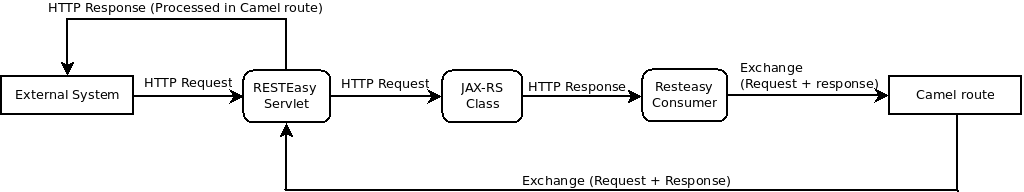
\includegraphics[width=1.1\linewidth]{diagrams/basic.png}
\caption{DFD illustrating Resteasy Consumer}
\label{dfd-basic}
\end{figure}


\begin{figure}[H]
%\advance\leftskip-0.5cm
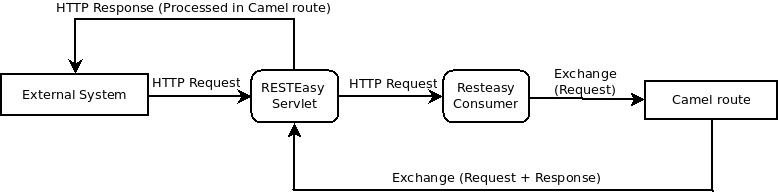
\includegraphics[width=1.0\linewidth]{diagrams/camelProxy.png}
\caption{DFD illustrating Resteasy Camel Proxy Consumer}
\label{dfd-camel}
\end{figure}


\begin{figure}[H]
%\advance\leftskip-2cm
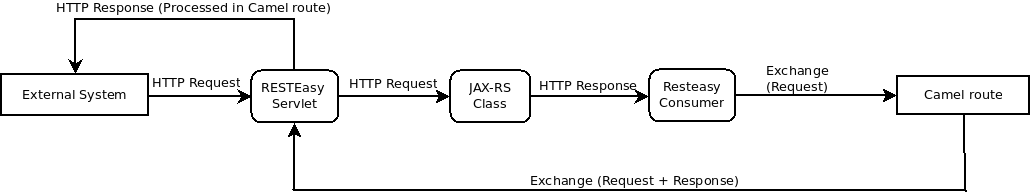
\includegraphics[width=1.1\linewidth]{diagrams/proxy.png}
\caption{DFD illustrating Resteasy Proxy Consumer}
\label{dfd-proxy}
\end{figure}

\begin{figure}[H]
%\advance\leftskip-1cm
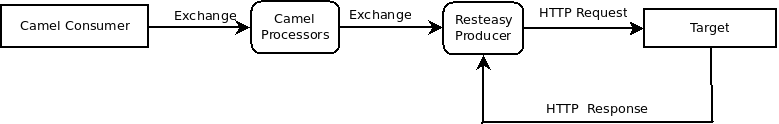
\includegraphics[width=1.0\linewidth]{diagrams/producer.png}
\caption{DFD illustrating Resteasy Producer}
\label{dfd-prod}
\end{figure}

%\section{Class Diagram}
\begin{figure}[H]\
\centering

\label{class-bla}
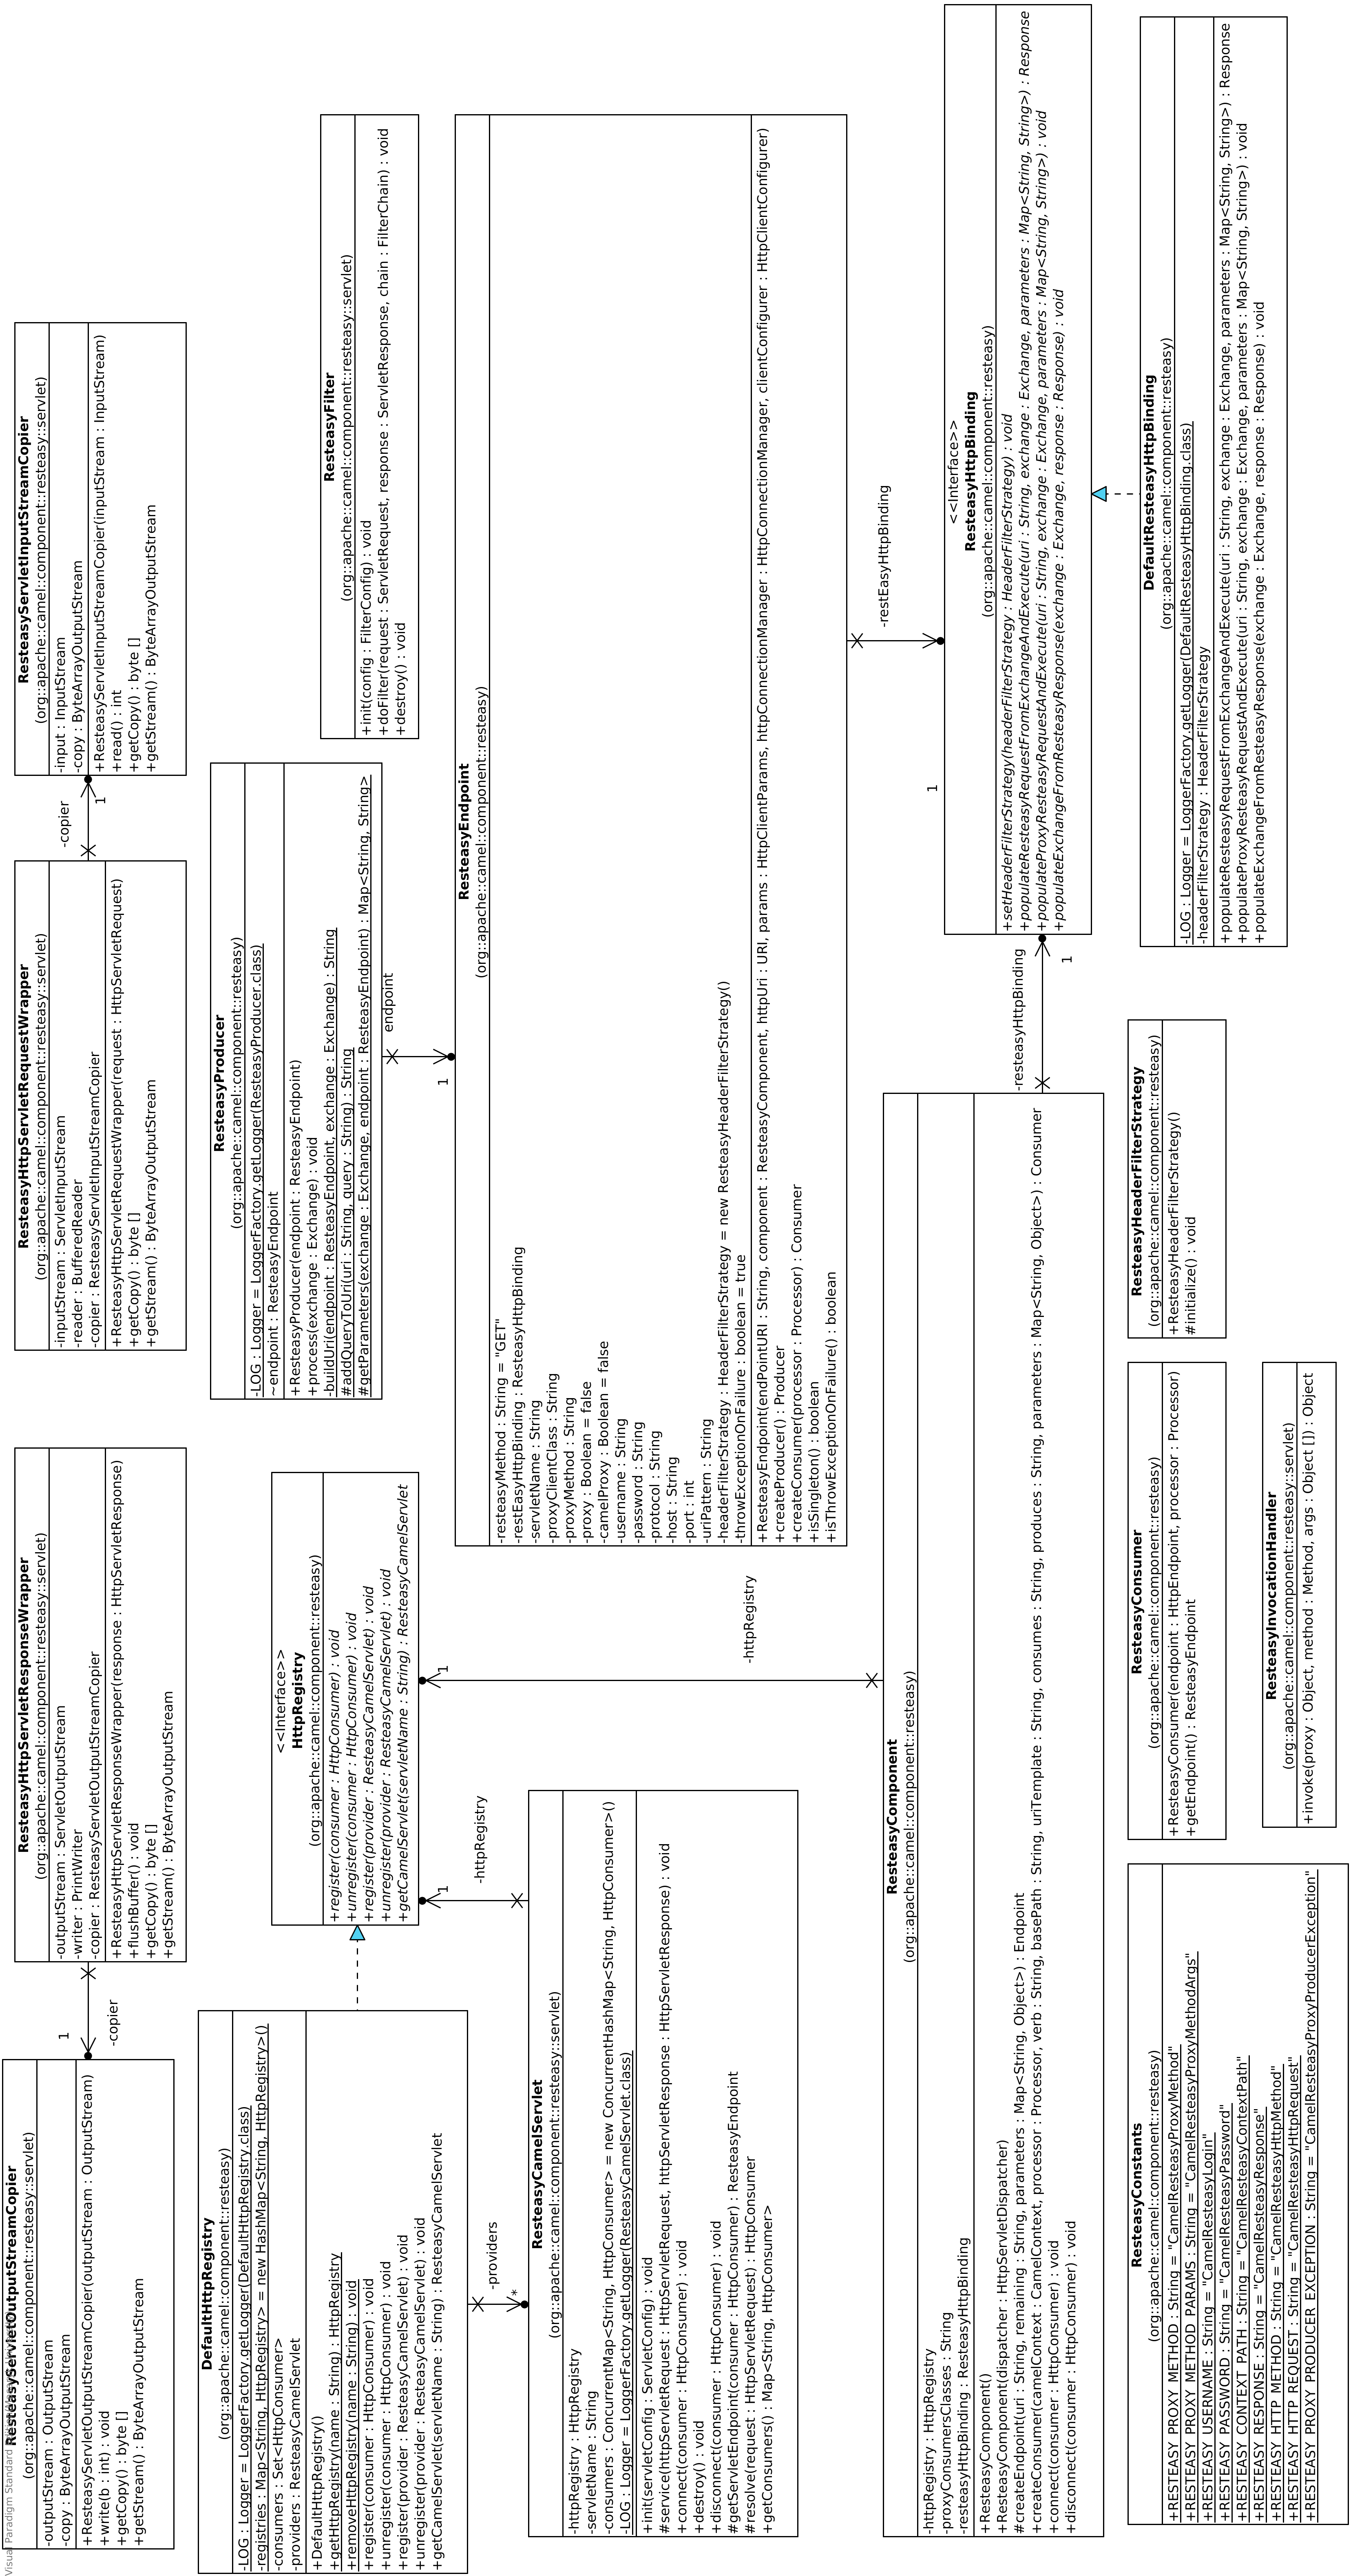
\includegraphics[width=1.0\linewidth , height=1.05\textheight]{diagrams/class2.png}

\end{figure}
%% End of the whole document
\end{document}